%%%%%%%%%%%%%%%%%%%%%%%%%%%%%%%%%%%%%%%%%
% Beamer Presentation
% LaTeX Template
% Version 1.0 (10/11/12)
%
% This template has been downloaded from:
% http://www.LaTeXTemplates.com
%
% License:
% CC BY-NC-SA 3.0 (http://creativecommons.org/licenses/by-nc-sa/3.0/)
%
%%%%%%%%%%%%%%%%%%%%%%%%%%%%%%%%%%%%%%%%%

%----------------------------------------------------------------------------------------
%	PACKAGES AND THEMES
%----------------------------------------------------------------------------------------

\documentclass{beamer}

\mode<presentation> {

% The Beamer class comes with a number of default slide themes
% which change the colors and layouts of slides. Below this is a list
% of all the themes, uncomment each in turn to see what they look like.

%\usetheme{default}
%\usetheme{AnnArbor}
%\usetheme{Antibes}
%\usetheme{Bergen}
%\usetheme{Berkeley}
%\usetheme{Berlin}
%\usetheme{Boadilla}
%\usetheme{CambridgeUS}
%\usetheme{Copenhagen}
%\usetheme{Darmstadt}
\usetheme{Dresden}
%\usetheme{Frankfurt}
%\usetheme{Goettingen}
%\usetheme{Hannover}
%\usetheme{Ilmenau}
%\usetheme{JuanLesPins}
%\usetheme{Luebeck}
%\usetheme{Madrid}
%\usetheme{Malmoe}
%\usetheme{Marburg}
%\usetheme{Montpellier}
%\usetheme{PaloAlto}
%\usetheme{Pittsburgh}
%\usetheme{Rochester}
%\usetheme{Singapore}
%\usetheme{Szeged}
%\usetheme{Warsaw}

% As well as themes, the Beamer class has a number of color themes
% for any slide theme. Uncomment each of these in turn to see how it
% changes the colors of your current slide theme.

%\usecolortheme{albatross}
%\usecolortheme{beaver}
%\usecolortheme{beetle}
%\usecolortheme{crane}
%\usecolortheme{dolphin}
%\usecolortheme{dove}
%\usecolortheme{fly}
%\usecolortheme{lily}
%\usecolortheme{orchid}
%\usecolortheme{rose}
%\usecolortheme{seagull}
%\usecolortheme{seahorse}
%\usecolortheme{whale}
%\usecolortheme{wolverine}

%\setbeamertemplate{footline} % To remove the footer line in all slides uncomment this line
%\setbeamertemplate{footline}[page number] % To replace the footer line in all slides with a simple slide count uncomment this line

%\setbeamertemplate{navigation symbols}{} % To remove the navigation symbols from the bottom of all slides uncomment this line
}

\usepackage{graphicx} % Allows including images
\usepackage{booktabs} % Allows the use of \toprule, \midrule and \bottomrule in tables

%----------------------------------------------------------------------------------------
%	TITLE PAGE
%----------------------------------------------------------------------------------------

\title[Design Phase]{Obstacle Avoidance and Goal Detection Robot using RPi and LRF.} % The short title appears at the bottom of every slide, the full title is only on the title page

\author{Atabak Hafeez \and
Maria Ficiu \and
Rubin Deliallisi \and
Siddharth Shukla} % Your name
\institute[Jacobs University Bremen] % Your institution as it will appear on the bottom of every slide, may be shorthand to save space
{
Jacobs University Bremen \\ % Your institution for the title page
\medskip
%\textit{john@smith.com} % Your email address
}
\date{\today} % Date, can be changed to a custom date

\begin{document}

\begin{frame}
\titlepage % Print the title page as the first slide
\end{frame}

\begin{frame}
\frametitle{Overview} % Table of contents slide, comment this block out to remove it
\tableofcontents % Throughout your presentation, if you choose to use \section{} and \subsection{} commands, these will automatically be printed on this slide as an overview of your presentation
\end{frame}


%----------------------------------------------------------------------------------------
%	PRESENTATION SLIDES
%----------------------------------------------------------------------------------------

%------------------------------------------------
\section{Introduction}
%------------------------------------------------

\subsection{Goal}
\begin{frame}
\frametitle{Goal (Basic)}
Given a goal:
\begin{itemize}
\item Turn the robot around
\item Move towards the goal based on the LRF input.
\item Example requirement: recommend new connections, movies, music.
\item How: using a genetic algorithm (more details later).
\end{itemize}
\end{frame}

\begin{frame}
\frametitle{More about Clustering}
\begin{itemize}
\item  	\textbf{Important terms}
\begin{description}
\item[Clusters] Subsets in which a given set of objects (in our case the nodes in the social network graph) is divided, such that the objects from the same subset are more similar to the objects from different subsets.
\item[Population] A set of solutions to the clustering problem.
\item[Individual] One solution to the clustering problem.
\end{description}
\end{itemize}
\end{frame}

\subsection{Architecture}
\begin{frame}
\frametitle{Sequence Diagram}
\begin{figure}[H]
\centering
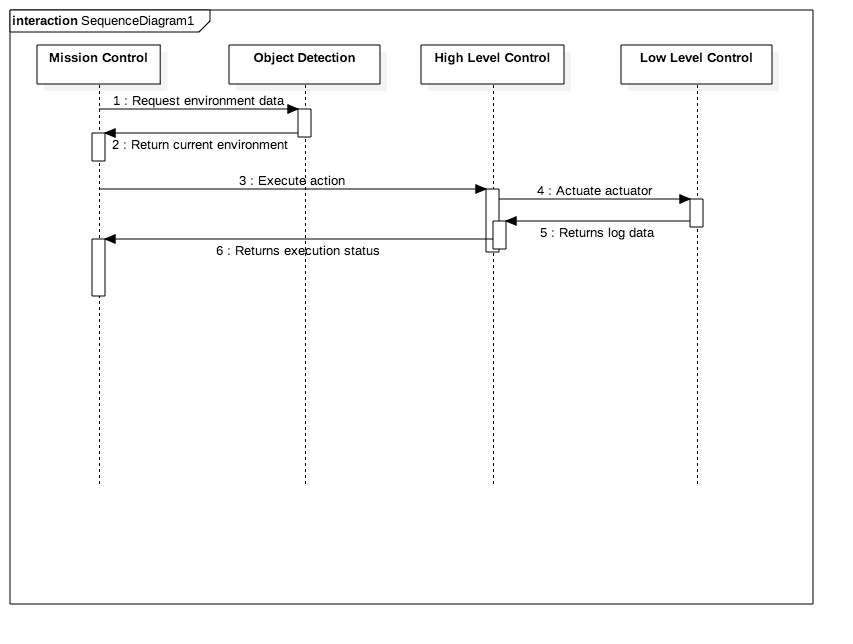
\includegraphics[scale=0.36]{assets/diagrams/SequenceDiagram.png}
%\caption{Displayes object interactions arranged in a time sequence.}
\end{figure}
\end{frame}

\begin{frame}
\frametitle{Component Diagram}
\begin{figure}[H]
\centering
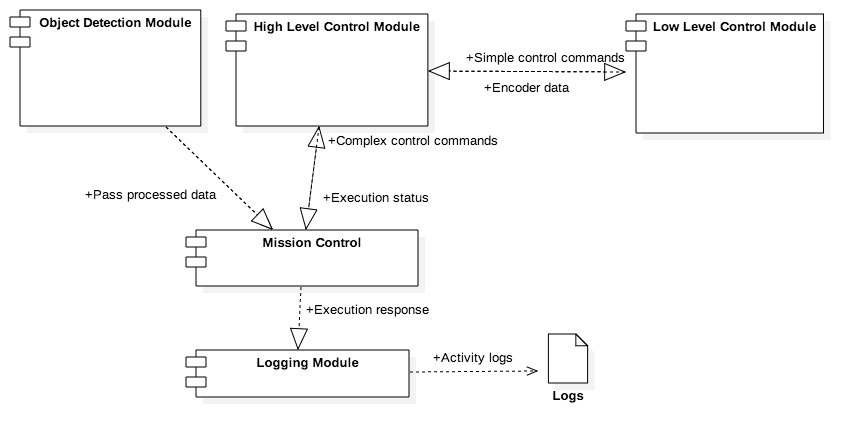
\includegraphics[scale=0.36]{assets/diagrams/ComponentDiagram.png}
%\caption{Shows how component are connected together.}
\end{figure}
\end{frame}

%------------------------------------------------
\section{Algorithm}
%------------------------------------------------


%------------------------------------------------
\section{Development Strategy}
%------------------------------------------------
\subsection{Testing}
\begin{frame}
\frametitle{Testing}
\begin{itemize}
\item Test Driven Development (TDD)
\begin{itemize}
\item Write tests before code
\item Helps clearly plan out program functionality
\item Reduces debug time drastically
\end{itemize}
\item Focused on four different domains:
\begin{itemize}
\item Unit Testing
\item Integration Testing 
\item System Testing
\item Stress Testing 
\end{itemize}
\end{itemize}
\end{frame}


%----------------------------------------------------------------------------------------
\end{document} 
